Loads represent the demand connected to the electrical network. In dynamic simulations they are modelled as algebraic or differential-algebraic components that transform the local bus voltage into either injected power or injected current. The sign convention used in the VeraGrid templates follows the network-injection formulation: consumed active and reactive power are represented as negative injections when the model is coupled to the grid.

The load models considered here cover RMS phasor-domain loads and EMT phase-domain ZIP loads. The RMS models are connected to the positive-sequence grid through phasor quantities or voltage magnitudes, while the EMT model is phase-selective and can be connected phase-to-ground or phase-to-phase depending on the selected shunt topology.

\section{RMS Phasor Current Load}

This model represents a constant-power load in RMS current-balance phasor coordinates. The terminal voltage is expressed as
\begin{equation}
    V = V_r + j V_i,
\end{equation}
and the injected current is
\begin{equation}
    I = I_r + j I_i.
\end{equation}

\begin{table}[H]
    \centering
    \caption{Variables of the RMS phasor current load.}
    \begin{tabular}{ll}
        \toprule
        Symbol & Description \\
        \midrule
        $V_r$, $V_i$ & Real and imaginary parts of the terminal voltage \\
        $I_r$, $I_i$ & Real and imaginary parts of the injected current \\
        $v_{r,aux}$, $v_{i,aux}$ & Auxiliary voltage variables used to write the current equations without division \\
        $V^2$ & Squared voltage magnitude used in the algebraic current equations \\
        \bottomrule
    \end{tabular}
\end{table}

\begin{table}[H]
    \centering
    \caption{Parameters of the RMS phasor current load.}
    \begin{tabular}{ll}
        \toprule
        Symbol & Description \\
        \midrule
        $P_{l0}$ & Active-power set-point in injection convention \\
        $Q_{l0}$ & Reactive-power set-point in injection convention \\
        $S_l$ & Complex load-power set-point, $S_l=P_{l0}+jQ_{l0}$ \\
        \bottomrule
    \end{tabular}
\end{table}

\paragraph{Base equations.}
The model keeps the active and reactive power set-points constant,
\begin{equation}
    S_l = P_{l0} + j Q_{l0},
\end{equation}
and computes the current injection from
\begin{equation}
    I = \overline{\frac{S_l}{V}}.
\end{equation}

\paragraph{Current-balance reformulation.}
For this model, the grid-interface equations and the multilinear-oriented form are naturally coupled. To avoid an explicit division in the algebraic system, the implemented equations use auxiliary voltage variables
\begin{equation}
    v_{r,aux}=V_r, \qquad v_{i,aux}=V_i,
\end{equation}
and
\begin{equation}
    V^2 = V_r v_{r,aux} + V_i v_{i,aux}.
\end{equation}
The current equations are then written as
\begin{align}
    I_r V^2 &= P_{l0} V_r + Q_{l0} V_i, \\
    I_i V^2 &= P_{l0} V_i - Q_{l0} V_r.
\end{align}
During initialization, the load powers are obtained from the power-flow current and voltage as
\begin{align}
    P_{l0} &= V_r I_r + V_i I_i, \\
    Q_{l0} &= V_i I_r - V_r I_i.
\end{align}

\paragraph{Grid connection.}
The model is connected to the RMS network through the real and imaginary parts of the bus voltage, $V_r$ and $V_i$. Its outputs are the current-injection components $I_r$ and $I_i$, which are mapped directly into the network current-balance equations. Load consumption is therefore represented by negative values of $P_{l0}$ and $Q_{l0}$ in the injection convention.

\section{EMT ZIP Load}

The EMT ZIP load is a phase-selective model. It can instantiate only the active phases present at the connection point and applies the same ZIP coefficient set to each active phase. For each phase or delta branch $x$, the instantaneous terminal voltage is denoted by $v_x$.

\begin{table}[H]
    \centering
    \caption{Variables of the EMT ZIP load for each active phase or branch $x$.}
    \begin{tabular}{ll}
        \toprule
        Symbol & Description \\
        \midrule
        $v_x$ & Instantaneous terminal voltage \\
        $u_x$, $q_x$ & SOGI direct and orthogonal voltage states \\
        $V_x^2$ & Squared voltage magnitude \\
        $V_{m,x}$ & Regularized voltage magnitude \\
        $r_x$ & Normalized voltage ratio \\
        $u_{aux,x}$, $q_{aux,x}$ & Auxiliary copies of the SOGI states used in the multilinear form \\
        $V_{m,aux,x}$, $r_{aux,x}$ & Auxiliary copies of voltage magnitude and voltage ratio \\
        $V^{-2}_{aux,x}$ & Auxiliary reciprocal of the regularized squared voltage magnitude \\
        $P_x$, $Q_x$ & Active and reactive ZIP power injections \\
        $i_x$ & EMT current injection \\
        \bottomrule
    \end{tabular}
\end{table}

\begin{table}[H]
    \centering
    \caption{Parameters of the EMT ZIP load.}
    \begin{tabular}{ll}
        \toprule
        Symbol & Description \\
        \midrule
        $P_{0,x}$ & Nominal active-power set-point for phase or branch $x$ \\
        $Q_{0,x}$ & Nominal reactive-power set-point for phase or branch $x$ \\
        $V_0$ & Nominal peak voltage used to normalize the ZIP polynomial \\
        $a_1$, $a_2$, $a_3$ & Active-power ZIP coefficients for impedance, current, and power terms \\
        $a_4$, $a_5$, $a_6$ & Reactive-power ZIP coefficients for impedance, current, and power terms \\
        $k_{sogi}$ & SOGI gain \\
        $\omega$ & Electrical angular frequency \\
        $\varepsilon$ & Small regularization parameter for magnitude and current equations \\
        \bottomrule
    \end{tabular}
\end{table}

\paragraph{Base equations.}
Each active phase uses a second-order generalized integrator (SOGI) to obtain an orthogonal voltage pair $(u_x,q_x)$ from the instantaneous voltage:
\begin{align}
    \dot{u}_x &= k_{sogi}\omega\left(v_x-u_x\right)-\omega q_x, \\
    \dot{q}_x &= \omega u_x.
\end{align}
The squared voltage magnitude, magnitude, and normalized voltage ratio are
\begin{align}
    V_x^2 &= u_x^2 + q_x^2, \\
    V_{m,x} &= \sqrt{u_x^2+q_x^2+\varepsilon}, \\
    r_x &= \frac{V_{m,x}}{V_0}.
\end{align}
The active and reactive ZIP powers are
\begin{align}
    P_x + P_{0,x}\left(a_1 r_x^2+a_2 r_x+a_3\right) &= 0, \\
    Q_x + Q_{0,x}\left(a_4 r_x^2+a_5 r_x+a_6\right) &= 0.
\end{align}
The corresponding current injection is calculated as
\begin{equation}
    i_x + \frac{2\left[u_x\left(-P_x\right)+q_x\left(-Q_x\right)\right]}{u_x^2+q_x^2+\varepsilon}=0.
\end{equation}
The small parameter $\varepsilon$ regularizes the magnitude and current equations during Newton iterations.

\paragraph{Multilinear reformulation.}
The EMT ZIP load also has a multilinear-oriented implementation in which powers, square roots, and divisions are replaced by auxiliary algebraic variables. The same SOGI states are kept, but duplicated variables are introduced,
\begin{equation}
    u_{aux,x}=u_x, \qquad q_{aux,x}=q_x,
\end{equation}
so that the squared voltage is written as
\begin{equation}
    V_x^2 = u_x u_{aux,x}+q_x q_{aux,x}.
\end{equation}
The voltage magnitude and normalized ratio are represented with auxiliary products,
\begin{align}
    V_{m,x} V_{m,aux,x} &= V_x^2+\varepsilon, \\
    r_x V_0 &= V_{m,x}, \\
    r_{aux,x} &= r_x.
\end{align}
The ZIP powers then become
\begin{align}
    P_x + P_{0,x}\left(a_1 r_x r_{aux,x}+a_2 r_x+a_3\right) &= 0, \\
    Q_x + Q_{0,x}\left(a_4 r_x r_{aux,x}+a_5 r_x+a_6\right) &= 0.
\end{align}
Finally, the current equation uses a reciprocal auxiliary variable,
\begin{align}
    V^{-2}_{aux,x}\left(V_x^2+\varepsilon\right) &= 1, \\
    i_x + 2\left[u_x\left(-P_x\right)+q_x\left(-Q_x\right)\right]V^{-2}_{aux,x} &= 0.
\end{align}
This form preserves the physical ZIP equations while exposing the nonlinear products through explicit auxiliary constraints.

\paragraph{Grid connection.}
The model exposes only the voltages and currents of the active phase set. With a ground-referenced connection, the inputs are the phase-to-ground voltages $v_A$, $v_B$, and $v_C$ for the enabled phases, and the outputs are the corresponding current injections $i_A$, $i_B$, and $i_C$. With a delta connection, the core ZIP equations are driven by line-to-line branch voltages. In that case the nominal peak voltage is scaled from $\sqrt{2}$ to $\sqrt{6}$, which accounts for the $\sqrt{3}$ ratio between line-to-line and phase-to-neutral voltage magnitudes. The wrapper then maps the branch currents back to the terminal phase currents injected into the EMT network.

\section{RMS ZIP Load}

The RMS ZIP load represents the consumed power as a polynomial function of the RMS voltage magnitude. It combines constant-impedance, constant-current, and constant-power behaviour.

\begin{table}[H]
    \centering
    \caption{Variables of the RMS ZIP load.}
    \begin{tabular}{ll}
        \toprule
        Symbol & Description \\
        \midrule
        $V_m$ & Local RMS voltage magnitude \\
        $r$ & Normalized voltage ratio, $r=V_m/V_0$ \\
        $r_{aux}$ & Auxiliary copy of $r$ used in the multilinear form \\
        $P$ & Active-power injection \\
        $Q$ & Reactive-power injection \\
        \bottomrule
    \end{tabular}
\end{table}

\begin{table}[H]
    \centering
    \caption{Parameters of the RMS ZIP load.}
    \begin{tabular}{ll}
        \toprule
        Symbol & Description \\
        \midrule
        $P_0$ & Nominal active-power set-point at $V_0$ \\
        $Q_0$ & Nominal reactive-power set-point at $V_0$ \\
        $V_0$ & Initial voltage magnitude used as the ZIP voltage reference \\
        $a_1$, $a_2$, $a_3$ & Active-power ZIP coefficients for impedance, current, and power terms \\
        $a_4$, $a_5$, $a_6$ & Reactive-power ZIP coefficients for impedance, current, and power terms \\
        \bottomrule
    \end{tabular}
\end{table}

\paragraph{Base equations.}
Let $V_m$ be the local RMS voltage magnitude and $V_0$ the initialization voltage. The normalized voltage ratio is
\begin{equation}
    r = \frac{V_m}{V_0}.
\end{equation}
The active and reactive powers are
\begin{align}
    P &= P_0\left(a_1 r^2+a_2 r+a_3\right), \\
    Q &= Q_0\left(a_4 r^2+a_5 r+a_6\right).
\end{align}
The coefficients $a_1$ and $a_4$ define the constant-impedance contribution, $a_2$ and $a_5$ the constant-current contribution, and $a_3$ and $a_6$ the constant-power contribution. They are required to satisfy
\begin{align}
    a_1+a_2+a_3 &= 1, \\
    a_4+a_5+a_6 &= 1.
\end{align}
In the template, the default coefficient split is $0.1$ impedance, $0.1$ current, and $0.8$ power for both active and reactive power.

\paragraph{Multilinear reformulation.}
The nonlinearity of the RMS ZIP model appears in the squared voltage-ratio terms. A multilinear-oriented form introduces auxiliary copies of the normalized voltage,
\begin{equation}
    r_{aux}=r,
\end{equation}
and rewrites the active and reactive powers as
\begin{align}
    P &= P_0\left(a_1 r r_{aux}+a_2 r+a_3\right), \\
    Q &= Q_0\left(a_4 r r_{aux}+a_5 r+a_6\right).
\end{align}
If $V_0$ is treated as a fixed parameter after initialization, the relation $r=V_m/V_0$ is affine in $V_m$. If $V_0$ is retained as a variable, an additional product relation $rV_0=V_m$ is used to avoid division.

\paragraph{Grid connection.}
The model is connected to the RMS network through the bus voltage magnitude $V_m$. Its outputs are the algebraic active and reactive power injections $P$ and $Q$, which are mapped to the network power-balance equations. The reference voltage $V_0$ is initialized from the connected bus voltage magnitude so that $P=P_0$ and $Q=Q_0$ at the initial operating point.

\section{Exponential Load}

The exponential load represents voltage-sensitive demand with active and reactive powers that vary as powers of the terminal voltage. It is a compact alternative to the ZIP model when the load response is better represented by fitted voltage exponents.

\begin{table}[H]
    \centering
    \caption{Variables of the exponential load models.}
    \begin{tabular}{ll}
        \toprule
        Symbol & Description \\
        \midrule
        $V_m$ & RMS voltage magnitude in the RMS model \\
        $v_x$ & Instantaneous EMT terminal voltage for phase or branch $x$ \\
        $u_x$, $q_x$ & EMT SOGI direct and orthogonal voltage states \\
        $V_{m,x}$ & EMT voltage magnitude for phase or branch $x$ \\
        $r$, $r_x$ & Normalized voltage ratios \\
        $r_{aux}$ & Auxiliary voltage-ratio copy used when integer exponents are expanded \\
        $V^{-2}_{aux,x}$ & Auxiliary EMT reciprocal voltage term used in tensor-compatible current equations \\
        $P$, $Q$ & RMS active and reactive power injections \\
        $P_x$, $Q_x$ & EMT active and reactive power injections for phase or branch $x$ \\
        $i_x$ & EMT current injection \\
        \bottomrule
    \end{tabular}
\end{table}

\begin{table}[H]
    \centering
    \caption{Parameters of the exponential load models.}
    \begin{tabular}{ll}
        \toprule
        Symbol & Description \\
        \midrule
        $P_0$, $Q_0$ & Nominal RMS active and reactive power set-points \\
        $P_{0,x}$, $Q_{0,x}$ & Nominal EMT active and reactive power set-points for phase or branch $x$ \\
        $V_0$ & Voltage reference used to normalize the voltage magnitude \\
        $a$ or $\alpha_p$ & Active-power voltage exponent \\
        $b$ or $\alpha_q$ & Reactive-power voltage exponent \\
        $k_{sogi}$ & EMT SOGI gain \\
        $\omega$ & EMT electrical angular frequency \\
        $\varepsilon$ & EMT regularization parameter for voltage magnitude \\
        \bottomrule
    \end{tabular}
\end{table}

\paragraph{Base equations.}
In the RMS model, the normalized voltage ratio is
\begin{equation}
    r = \frac{V_m}{V_0}.
\end{equation}
The active and reactive power injections are
\begin{align}
    P &= P_0 r^a, \\
    Q &= Q_0 r^b.
\end{align}
In the EMT model, each active phase or branch first computes the same SOGI states as the EMT ZIP load,
\begin{align}
    \dot{u}_x &= k_{sogi}\omega\left(v_x-u_x\right)-\omega q_x, \\
    \dot{q}_x &= \omega u_x,
\end{align}
and then evaluates
\begin{align}
    V_x^2 &= u_x^2 + q_x^2, \\
    V_{m,x} &= \sqrt{\left|V_x^2\right|+\varepsilon}, \\
    r_x &= \frac{V_{m,x}}{V_0}.
\end{align}
The EMT exponential powers and current injection are
\begin{align}
    P_x + P_{0,x} r_x^{\alpha_p} &= 0, \\
    Q_x + Q_{0,x} r_x^{\alpha_q} &= 0, \\
    i_x - \frac{2\left(u_x P_x + q_x Q_x\right)}{\left|V_x^2\right|+\varepsilon} &= 0.
\end{align}

\paragraph{Multilinear reformulation.}
The exponential model cannot be made multilinear exactly for arbitrary real-valued exponents. The base equations are therefore written first, and the reformulation depends on the selected exponents. If the exponents are fixed integers, the powers can be expanded with auxiliary copies. For example, for $a=b=2$,
\begin{equation}
    r_{aux}=r,
\end{equation}
and
\begin{align}
    P &= P_0 r r_{aux}, \\
    Q &= Q_0 r r_{aux}.
\end{align}
For general exponents, the usual tensor-compatible approach is to approximate $r^a$ and $r^b$ with a polynomial, piecewise-polynomial, or lookup-based representation, and then introduce auxiliary variables for the resulting products. The EMT version requires the same auxiliary treatment used by the EMT ZIP model for voltage magnitude and reciprocal-current terms before applying the exponent approximation.

\paragraph{Grid connection.}
The RMS exponential load connects through the RMS voltage magnitude $V_m$ and contributes $P$ and $Q$ to the power-balance equations. The EMT exponential load follows the same phase-selective connection structure as the EMT ZIP load: it can expose only the active phases, and it can be wrapped as a ground-referenced or delta-connected load. For delta connections, the voltage reference is scaled to the line-to-line peak voltage level.

\section{Motor Load}

Motor loads represent rotating electrical demand, typically induction motors. Unlike static ZIP or exponential loads, they include internal electrical states and mechanical speed dynamics, so they can capture fault response, stalling, and post-fault recovery behaviour.

\begin{figure}[H]
    \centering
    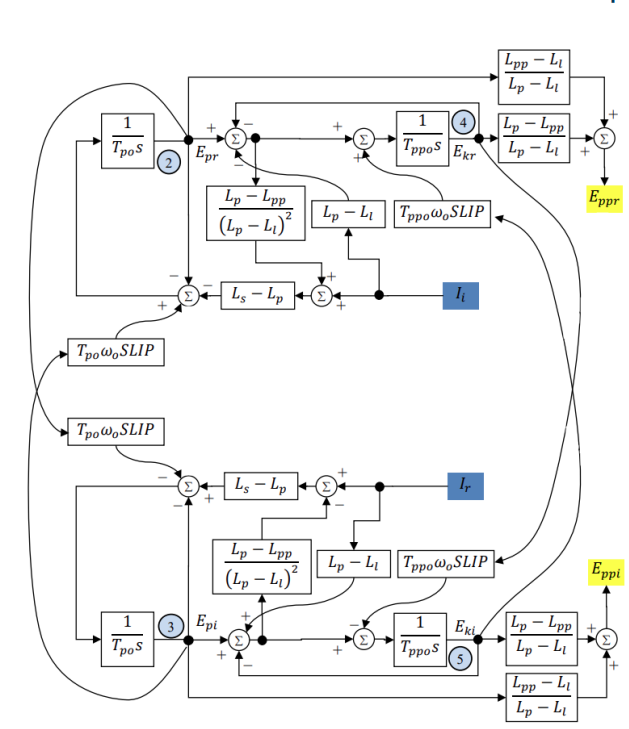
\includegraphics[width=0.9\textwidth]{pictures/loads/motor.png}
    \caption{Block diagram of the induction motor load model.}
    \label{fig:motor-load}
\end{figure}

\begin{table}[H]
    \centering
    \caption{Variables of the RMS induction motor load.}
    \begin{tabular}{ll}
        \toprule
        Symbol & Description \\
        \midrule
        $V_m$, $V_a$ & RMS terminal voltage magnitude and angle \\
        $V_d$, $V_q$ & Terminal voltage components in the motor reference frame \\
        $I_d$, $I_q$ & Motor current components in the motor reference frame \\
        $P$, $Q$ & Active and reactive power injections \\
        $E'_d$, $E'_q$ & Transient internal voltage states \\
        $E''_d$, $E''_q$ & Subtransient internal voltage states \\
        $\omega$ & Rotor speed \\
        $T_e$ & Electrical torque \\
        \bottomrule
    \end{tabular}
\end{table}

\begin{table}[H]
    \centering
    \caption{Parameters of the RMS induction motor load.}
    \begin{tabular}{ll}
        \toprule
        Symbol & Description \\
        \midrule
        $R_s$ & Stator resistance \\
        $L_s$ & Stator leakage inductance \\
        $L_p$ & Magnetizing inductance \\
        $L''$ & Subtransient inductance \\
        $T'_{p0}$ & Transient open-circuit time constant \\
        $T''_{p0}$ & Subtransient open-circuit time constant \\
        $H$ & Inertia constant \\
        $D$ & Damping coefficient \\
        $n$ & Mechanical load-torque speed exponent \\
        $C_{l0}$ & Initial mechanical load torque \\
        $\omega_s$ & Synchronous speed \\
        $\omega_0$ & Initial rotor speed used in the mechanical torque law \\
        $g$, $b$ & Optional shunt conductance and susceptance included with the motor load \\
        \bottomrule
    \end{tabular}
\end{table}

\paragraph{Base equations.}
The terminal voltage is transformed into the motor reference frame as
\begin{align}
    V_d &= -V_m\sin V_a, \\
    V_q &= V_m\cos V_a.
\end{align}
The motor slip is
\begin{equation}
    s = 1-\omega.
\end{equation}
The transient voltage dynamics are
\begin{align}
    \dot{E}'_d &= E'_q\omega_s s - \frac{I_q\left(L_s-L_p\right)+E'_d}{T'_{p0}}, \\
    \dot{E}'_q &= -E'_d\omega_s s - \frac{-I_d\left(L_s-L_p\right)+E'_q}{T'_{p0}}.
\end{align}
The subtransient equations use the transient states as driving quantities,
\begin{align}
    \dot{E}''_d &= -\left(E'_q-E''_q\right)\omega_s s - \frac{E'_d-E''_q-\left(L_p-L''\right)I_q}{T''_{p0}} + \dot{E}'_d, \\
    \dot{E}''_q &= \left(E'_d-E''_d\right)\omega_s s - \frac{E'_q-E''_d+\left(L_p-L''\right)I_d}{T''_{p0}} + \dot{E}'_q.
\end{align}
The algebraic stator equations are
\begin{align}
    V_d - E''_d + R_s I_d - L'' I_q &= 0, \\
    V_q - E''_q + R_s I_q + L'' I_d &= 0.
\end{align}
The active and reactive power injections are
\begin{align}
    P &= V_d I_d + V_q I_q - g V_m^2, \\
    Q &= V_q I_d - V_d I_q + b V_m^2.
\end{align}
The electrical torque and rotor-speed dynamics are
\begin{align}
    T_e &= E''_q I_q + E''_d I_d, \\
    \dot{\omega} &= \frac{T_e - C_{l0}\left|\omega/\omega_0\right|^n}{2H}.
\end{align}

\paragraph{Multilinear reformulation.}
The motor load is presented here in its physical dynamic form. A full multilinear reformulation would require auxiliary variables for the trigonometric voltage transformation, products between internal voltages and currents, and the nonlinear mechanical torque term. Since this is a high-order dynamic model, the reformulated version should be introduced separately only when the motor model is selected for tensor-based analysis.

\paragraph{Grid connection.}
The RMS motor load connects to the RMS network through $V_m$ and $V_a$ and contributes $P$ and $Q$ to the power-balance equations. Because the model includes rotor speed and internal voltage states, the injected power is not only a static function of voltage; it also depends on the motor's dynamic state after disturbances. EMT induction motor templates follow the same physical purpose but are represented directly in the phase-domain EMT formulation.

\section{Shunt Models}

Shunt devices represent passive elements connected between a network node and a reference node or between phases. They are commonly used to model fixed admittances, shunt compensation, reactors, capacitors, and equivalent passive demand components. In VeraGrid, shunts are available in both RMS and EMT formulations.

\subsection{RMS Shunt}

The RMS shunt is an admittance-based model defined by its conductance $g$ and susceptance $b$. Two equivalent RMS interfaces are available: a power-balance interface using voltage magnitude and angle, and a phasor current-balance interface using real and imaginary voltage components.

\begin{table}[H]
    \centering
    \caption{Variables of the RMS shunt models.}
    \begin{tabular}{ll}
        \toprule
        Symbol & Description \\
        \midrule
        $V_m$ & RMS voltage magnitude \\
        $V_{m,aux}$ & Auxiliary copy of $V_m$ used if $V_m^2$ is expanded as a product \\
        $V_a$ & RMS voltage angle \\
        $V_r$, $V_i$ & Real and imaginary parts of the RMS phasor voltage \\
        $P$, $Q$ & Active and reactive power injections \\
        $I_r$, $I_i$ & Real and imaginary parts of the injected current \\
        \bottomrule
    \end{tabular}
\end{table}

\begin{table}[H]
    \centering
    \caption{Parameters of the RMS shunt models.}
    \begin{tabular}{ll}
        \toprule
        Symbol & Description \\
        \midrule
        $g$ & Shunt conductance \\
        $b$ & Shunt susceptance \\
        \bottomrule
    \end{tabular}
\end{table}

\paragraph{Base equations.}
In the power-balance formulation, the shunt power injections are
\begin{align}
    P + g V_m^2 &= 0, \\
    Q - b V_m^2 &= 0.
\end{align}
In the phasor current-balance formulation, the injected current is computed from the terminal voltage as
\begin{align}
    I_r &= -g V_r + b V_i, \\
    I_i &= -g V_i - b V_r.
\end{align}
These equations are consistent with the same injection convention used by the load models.

\paragraph{Multilinear reformulation.}
No separate reformulation is required for the phasor current-balance shunt when $g$ and $b$ are parameters, because the current equations are linear in the voltage variables. For the power-balance form, the voltage-squared terms can be written with an auxiliary copy $V_{m,aux}=V_m$ as $V_mV_{m,aux}$ if the tensor formulation requires every repeated variable product to be explicit.

\paragraph{Grid connection.}
The power-balance RMS shunt connects through $V_m$ and $V_a$ and contributes $P$ and $Q$ to the RMS network equations. The phasor RMS shunt connects through $V_r$ and $V_i$ and contributes $I_r$ and $I_i$ to the current-balance network equations. The selected interface therefore follows the RMS network formulation used by the surrounding model.

\subsection{EMT RLC Shunt}

The EMT shunt templates model phase-selective passive $R$, $L$, and $C$ branches. The templates can be instantiated as individual resistor, inductor, or capacitor shunts, or as a combined RLC shunt where any subset of the three branches is enabled.

\begin{table}[H]
    \centering
    \caption{Variables of the EMT RLC shunt for each active phase or branch $x$.}
    \begin{tabular}{ll}
        \toprule
        Symbol & Description \\
        \midrule
        $v_x$ & Terminal voltage of phase or branch $x$ \\
        $v_N$ & Neutral voltage for star-connected variants \\
        $v_{drop,x}$ & Voltage across the shunt branch, $v_x-v_N$ for star connections \\
        $i_x$ & Total current injection of phase or branch $x$ \\
        $i_{L,x}$ & Inductor current state \\
        $v_{C,x}$ & Capacitor voltage state \\
        $i_N$ & Neutral current injection when the neutral is exposed \\
        \bottomrule
    \end{tabular}
\end{table}

\begin{table}[H]
    \centering
    \caption{Parameters of the EMT RLC shunt.}
    \begin{tabular}{ll}
        \toprule
        Symbol & Description \\
        \midrule
        $R_x$ & Resistance of phase or branch $x$ \\
        $L_x$ & Inductance of phase or branch $x$ \\
        $C_x$ & Capacitance of phase or branch $x$ \\
        $P_{l0,x}$ & Active-power reference used to initialize $R_x$ when no direct value is provided \\
        $Q_{l0,x}$ & Reactive-power reference used to initialize $L_x$ or $C_x$ when no direct value is provided \\
        $V_{nom}$ & Nominal voltage used for parameter initialization \\
        $\omega_{base}$ & Base angular frequency used for reactive-branch initialization \\
        \bottomrule
    \end{tabular}
\end{table}

\paragraph{Base equations.}
For a resistive shunt branch, the current equation is
\begin{equation}
    i_x + \frac{v_x}{R_x}=0.
\end{equation}
When the resistance is initialized from an active-power reference,
\begin{equation}
    R_x = \frac{V_{nom}^2}{P_{l0,x}}.
\end{equation}
For an inductive shunt branch, the current is a dynamic state and follows
\begin{equation}
    \dot{i}_{L,x} = -\frac{v_x}{L_x},
\end{equation}
with
\begin{equation}
    L_x = \frac{V_{nom}^2}{Q_{l0,x}\omega_{base}}.
\end{equation}
For a capacitive shunt branch, the capacitor voltage state is constrained to the terminal voltage and the current is computed from its derivative:
\begin{align}
    v_{C,x} - v_x &= 0, \\
    i_x + C_x \dot{v}_{C,x} &= 0,
\end{align}
with
\begin{equation}
    C_x = \frac{Q_{l0,x}}{V_{nom}^2\omega_{base}}.
\end{equation}
In the combined RLC model, the voltage across each branch is
\begin{equation}
    v_{drop,x}=v_x-v_N
\end{equation}
for star connections, and the total phase current equation combines the enabled branches as
\begin{equation}
    i_x + \frac{v_{drop,x}}{R_x} - i_{L,x} + C_x \dot{v}_{C,x}=0,
\end{equation}
where omitted branches are simply removed from the equation. The neutral node satisfies Kirchhoff's current law,
\begin{equation}
    i_N + \sum_x i_x = 0,
\end{equation}
with the grounding current included when the neutral is internally grounded.

\paragraph{Multilinear reformulation.}
The EMT RLC shunt is already linear in the electrical states when $R_x$, $L_x$, and $C_x$ are fixed parameters. If these parameters are retained as variables, the divisions used in the initialization formulas can be replaced by product constraints such as $R_xP_{l0,x}=V_{nom}^2$, $L_xQ_{l0,x}\omega_{base}=V_{nom}^2$, and $C_xV_{nom}^2\omega_{base}=Q_{l0,x}$. The dynamic branch equations themselves do not require an additional reformulation once the branch values are fixed.

\paragraph{Grid connection.}
The EMT shunts expose only the active phase set selected at template construction. Individual R, L, and C shunts connect each active phase directly to the EMT network and inject the corresponding phase currents. The combined RLC shunt supports grounded-star, neutral-star, floating-star, and delta connections. In grounded-star mode the neutral is tied to an internal ideal ground; in neutral-star mode the neutral is exposed as an additional terminal; in floating-star mode the neutral voltage is an internal algebraic variable constrained by neutral KCL; and in delta mode the branches are connected phase-to-phase and the resulting branch currents are mapped back to terminal phase-current injections.
